\section{COCOMO analysis}
The COCOMO model allows to estimate the time effort required by the project. We use the version of this model called COCOMO II. It is based on a main formula:
\begin{equation}
PM = A * Size^{E} * \prod_{1<=i<=n}^{} EM_{i} 
\end{equation}

where:
\begin{itemize}
	\item \textbf{PM} stands for "Person-Months"
	\item \textbf{A}=2.94. It approximates a productivity constant in PM/KSLOC for the case where E = 1.0.
	\item \textbf{Size} is measured in KSLOC and is the result of the Function Points analysis.
	\item \textbf{E} is an aggregation of 5 \textbf{scale factors}:
	\begin{itemize}[label = {-}]
		\item \textbf{Precedentedness:} It is high if the project is similar to several previous projects
		\item \textbf{Development Flexibility:} It is high if there are no specific constraints to conform to pre-established     requirements and external interface specifications.
		\item \textbf{Architecture / Risk Resolution:}It is high if the project plan includes a good risk management plan, a clear definition of budget and schedule, with a focus on architectural definition
		\item \textbf{Team Cohesion:} It is high if all stakeholders are able to work in a team and share the same vision and commitment.
		\item \textbf{Process Maturity:} Refers to a well known method for assessing the maturity of a software organization, CMMI, that is a process level improvement training and appraisal program.
	\end{itemize}
	\begin{figure}[H] 
		\centering
		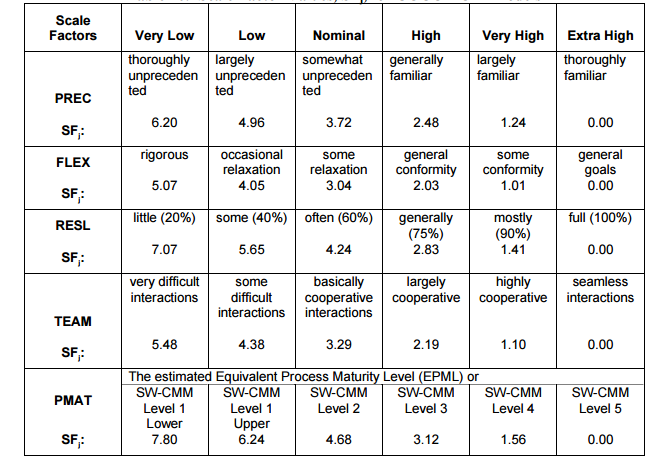
\includegraphics[scale = 0.7]{img/scaleFactors.png}
		\caption{Scale Factors}
	\end{figure}
	
	E is calculated with the formula:
	\begin{equation}
	E = B + 0.01 * \sum_{1<=j<=5}^{} SF_{j}
	\end{equation}
	where B=0.91
	
	\item\textbf{EM} stands for Effort Multiplier. Effort multipliers are derived from \textbf{Cost drivers}. The selection of these cost drivers depends on wh1ether the project regards a \textbf{Post-Architecture} system or a \textbf{Early Design} system. We are in the Early Design case, because we are extending an existing product and our system will be developed from scratch. So the cost drivers are:
	\begin{itemize}[label = {-}]
		\item {\textbf{Personnel Capability (PERS):} it is a combination of Analyst Capability(ACAP), Programmer Capability(PCAP) and Personnel Continuity cost driver of Post-Architecture.

			In our case we have little experience in the software analysis but this is balanced by good programming skills. The combination of ACAP and PCAP can be considered as \textbf{"Nominal"}
			
			\textbf{PERS=1.0}
\begin{figure}[H] 
	\centering
	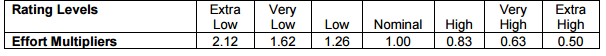
\includegraphics[scale = 0.6]{img/PERS.png}
	\caption{EMs of PERS}
\end{figure}
		
		}
		\item {\textbf{Product Reliability and Complexity(RCPX):} it is a combination of Required Software Reliability(RELY), Data Base Size(DATA), Product Complexity(CPLX) and Documentation Match to Life-Cycle Need(DOCU) cost drivers of Post-Architecture. 
			\\
			\\
			The software reliability is very important because a failure of the system can potentially cause a huge financial loss.\\
			The DATA cost driver attempts to capture the effect large test data requirements have on product development. For this particular driver we don’t have enough information to do a reliable estimation so the value can be considered \textbf{"Nominal"}.\\
			We decided to assign the complexity of the system a value \textbf{"Very high"}
			
		
			\textbf{RCPX=1.33}

\begin{figure}[H] 
	\centering
	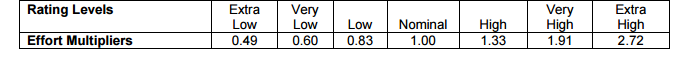
\includegraphics[scale = 0.6]{img/RCPX.png}
	\caption{EM of RCPX}
\end{figure}
	
		}
		
		\item {\textbf{Developed for Reusability(RUSE)}\\
			There are no requirement on Reusability so the value is considered \textbf{"Nominal"}
			
			\textbf{RUSE=1.0}
			
		\begin{figure}[H] 
			\centering
			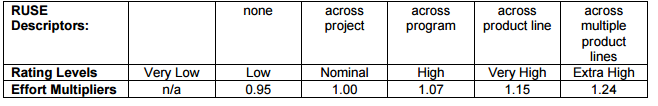
\includegraphics[scale = 0.6]{img/RUSE.png}
			\caption{EMs of RUSE}
		\end{figure}
		
		}
		\item{ \textbf{Platform Difficulty(PDIF): }it is a combination of Execution Time Constraint(TIME), Main Storage Constraint(STOR) and Platform Volatility(PVOL) cost drivers of Post-Architecture. 
		\\
		\\
		The OnBoard device is real-time embedded product so the execution time is important, but on the rest of the system there are no particular constraint about the execution time. Same as before there are no requirements on Storage.
		Platform Volatility can be considered \textbf{"Very high"} because the system is composed of different part on different system (OnBoard Device, Application Logic on server, Client on smartphone or browser).
		\\
		\textbf{PDIF=1.29}
		
		\begin{figure}[H] 
			\centering
			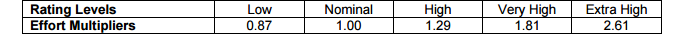
\includegraphics[scale = 0.6]{img/PDIF.png}
			\caption{EMs of PDIF}
		\end{figure}
	}
		\item {\textbf{Personnel Experience(PREX):} it is a combination of Application Experience(APEX), Platform Experience(PLEX), Language and Tool Experience(LTEX) cost drivers of Post-Architecture. 
			\\
			\\
			The overall experience is considered \textbf{"low" }
			\\
			\textbf{PREX=1.22}
		\begin{figure}[H] 
			\centering
			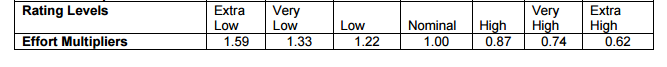
\includegraphics[scale = 0.6]{img/PREX.png}
			\caption{EMs of PREX}
		\end{figure}
	}
		\item {\textbf{Facilities(FCIL):} it is a combination of Use of Software Tools(TOOL) and Multisite Development(SITE) cost drivers of Post-Architecture. 
		\\
		\\
		Because of the entity and the life-cycle of the product development there are different system and tools that need to be integrated to develop the whole product so TOOL is considered \textbf{"Low"}.
		With all the new collaboration tools (Slack, github, Skype) the Multi-Site development driver is considered \textbf{"Nominal"}
		\\
		\textbf{FCIL=1.10}
		\begin{figure}[H] 
			\centering
			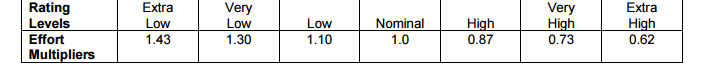
\includegraphics[scale = 0.6]{img/FCIL.png}
			\caption{EMs of FCIL}
		\end{figure}
	}
		\item {\textbf{Required Development Schedule(SCED)}
		\\
		\\
		Non accelerated Developement Schedule so it's considered \textbf{"Nominal"}.
		\\
		\textbf{SCED=1.0}
		
		\begin{figure}[H] 
			\centering
			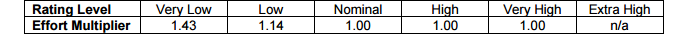
\includegraphics[scale = 0.6]{img/SCED.png}
			\caption{EMs of SCED}
		\end{figure}
	}
	\end{itemize} 
\end{itemize}



\begin{table}[]
	\centering
	\resizebox{\textwidth}{!}{%
		\begin{tabular}{lllllllll}
			\hline
			\textbf{Driver} & PERS & RCPX & RUSE & PDIF & PREX & FCIL & SCED & Product   \\ \hline
			\textbf{Value}  & 1.0  & 1.33 & 1.0  & 1.29 & 1.22 & 1.10 & 1.0  & 2.3024694 \\ \hline
		\end{tabular}%
	}
	\caption{EM Result Table}
\end{table}
\subsection{Results} 
According to the element in each section and their weight in complexity the total of th Function Points that provide an indication of the size of the system in functional terms:
1,33*1,29*1,22*1,1=2,3024694
\begin{equation}
EM=PERS * RCPX * RUSE * PDIF * PREX * FCIL * SCED \approx2.3
\end{equation}



